
The derivations in the previous section requiring little adjustment for accommodating a regressor and its corresponding varying slope function, as defined in Equation~\ref{eq:simplest_VC_model_mean} with $\mu\left(t\right) =  Q\alpha$, where 
\[
Q = \left[B | diag\left\{x\left(t\right) \right\}B \right]
\]
but now $B$ holds a rich B-spline basis with equally-spaced knots. If one wishes to allow for differing degrees of smoothing for each of the varying intercept term and the slope function, the P-spline objective function \ref{eq:S_pen_varying_intercept_model} must be further modified to accommodate multiple tuning parameters, $\lambda_i$, $i=0,1$. The objective function then becomes
\begin{align} 
\begin{split}
S^*_\lambda &= \vert y- Q\alpha  \vert^2  + \lambda_0 \vert D_{d_0} \alpha_0 \vert^2 + \lambda_1 \vert D_{d_1} \alpha_1 \vert^2\\
	&= \vert y- Q\alpha  \vert^2  + \vert \alpha^T P \alpha \vert^2
\end{split} \label{eq:S_pen_star}
\end{align}

where the penalty has form $P = \mbox{block diag}\left(\lambda_0 D_{d_0}^TD_{d_0}, \lambda_1 D_{d_1}^TD_{d_1} \right)$. The minimizer of \ref{eq:S_pen_star} is given by
\[
\hat{\alpha} = \left(Q^T Q +  P\right)^{-1}Q^T y.
\]

The block diagonal structure of the penalty separates the penalization of each individual smooth component. The estimated mean function is then given by 
\[
\hat{\mu} = Q \hat{\alpha} = H y
\] 
where
\begin{equation} \label{eq:simplest_VC_model_hat_matrix}
H = Q\left(Q^T Q +  P\right)^{-1}Q^T.
\end{equation}

{\needsparaphrased{[Figure~\ref{fig:PS_VCM_section_figure_1} Need to explain figure 3 here. ]} }

\begin{figure}[H]
   \graphicspath{{img/}}
   \centering
  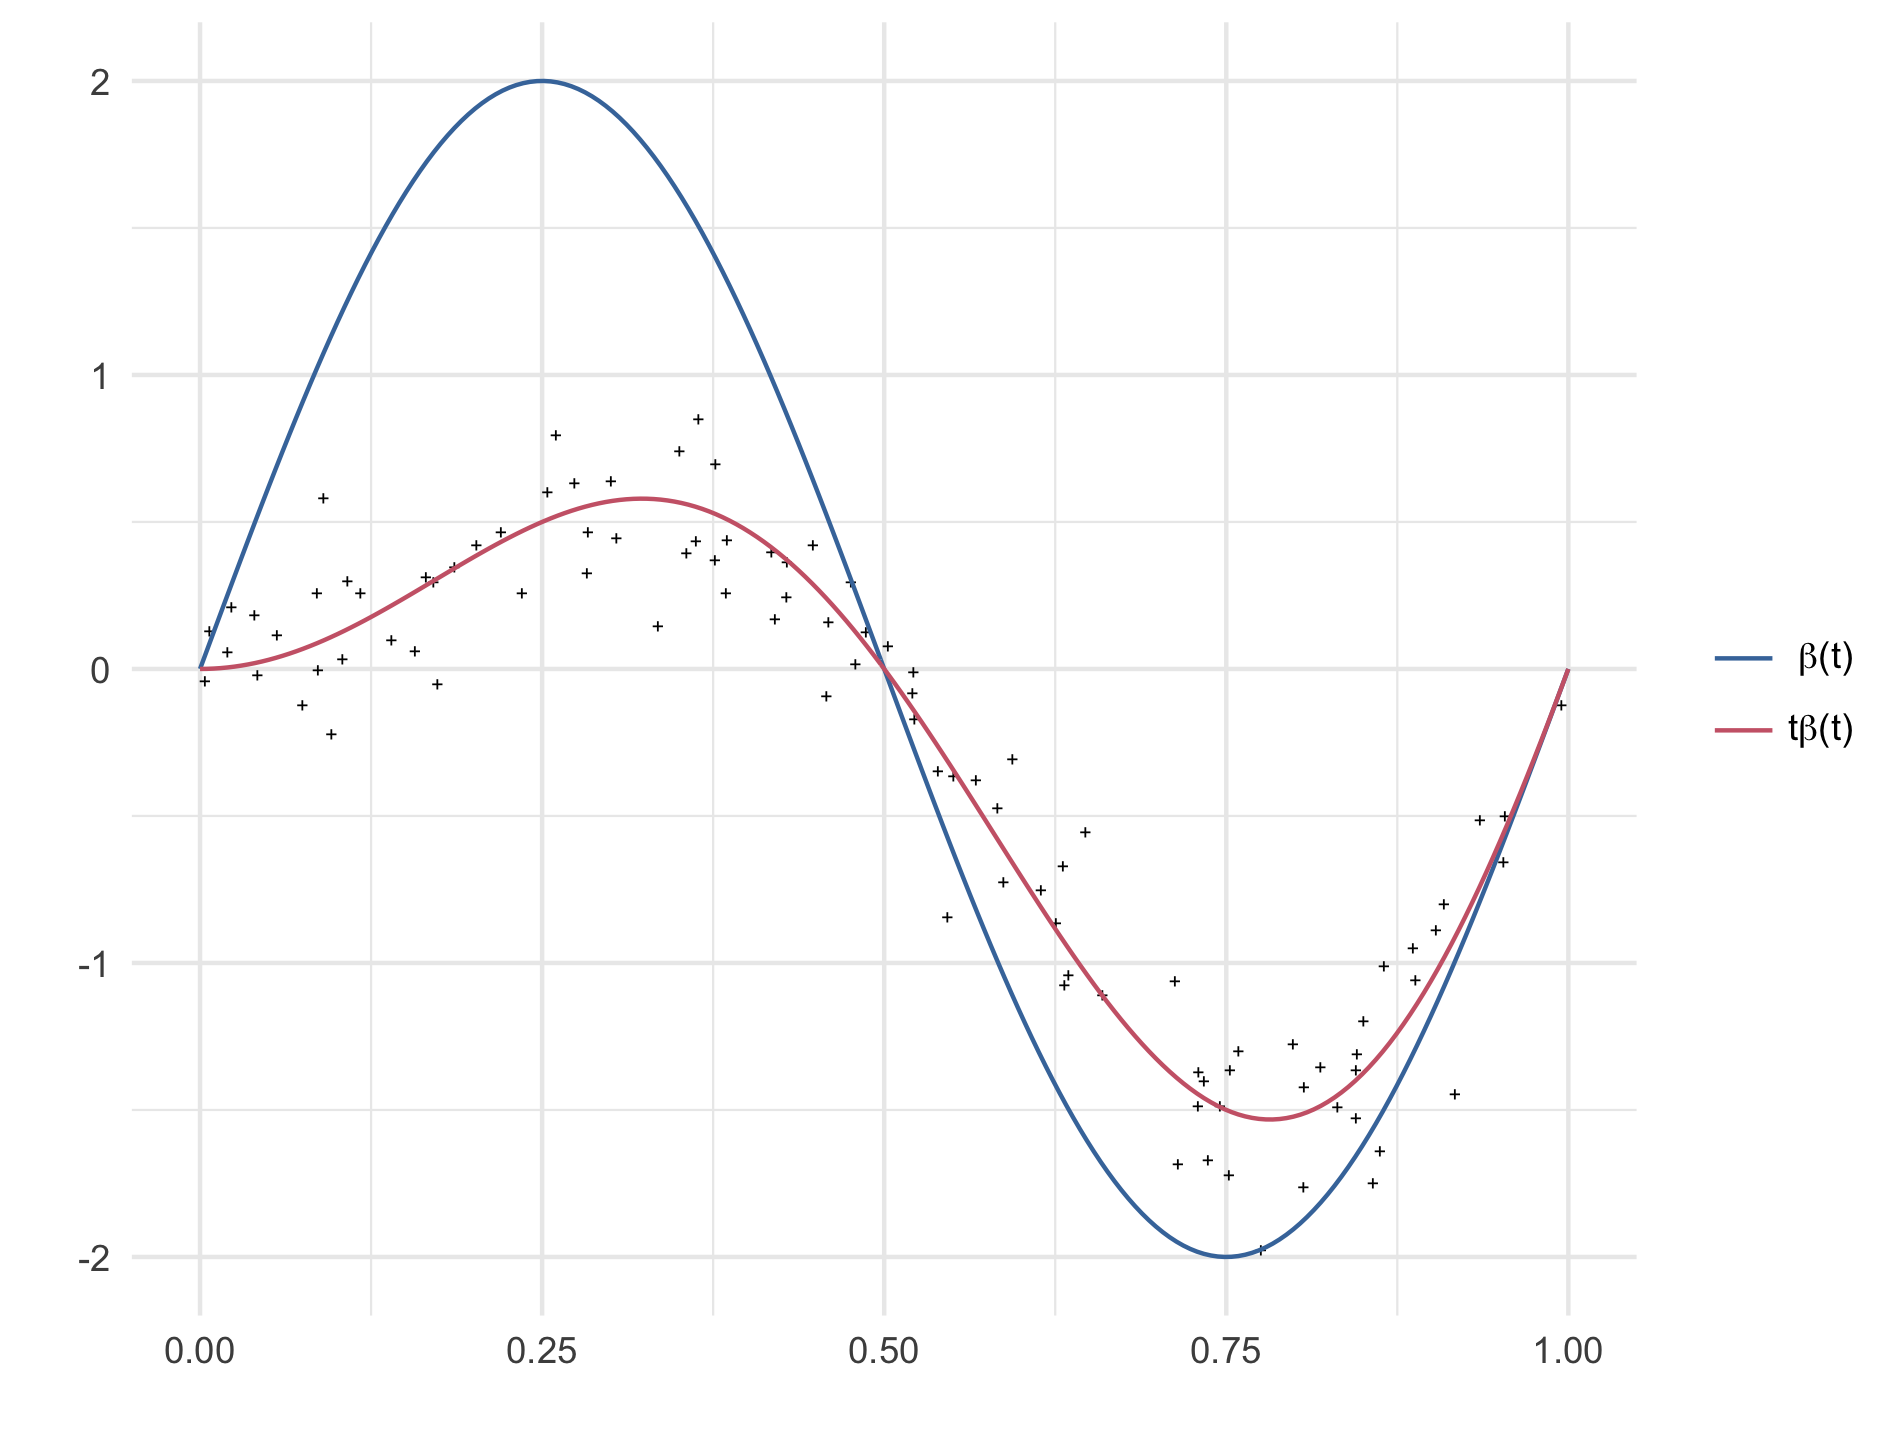
\includegraphics[scale=0.25]{PS_VCM_section_figure_1.png}
\caption{\textit{100 simulated data points where} $y\left(t\right) = t \beta\left( t \right) + 0.2\epsilon\left(t\right)$ \textit{where} $\epsilon$ \textit{is a white noise process with unit variance, and} $\beta\left(t\right) = 2\sin\left(2\pi t\right)$.}
\label{fig:PS_VCM_section_figure_1}
\end{figure}

\begin{figure}[H]
 \begin{subfigure}{.48\textwidth}
  \centering
   \graphicspath{{img/}}
 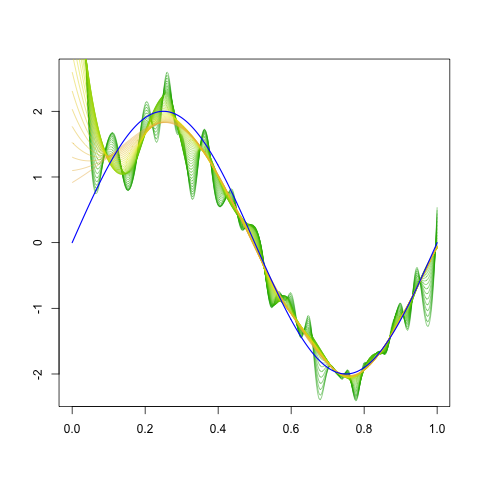
\includegraphics[scale=0.5]{PS_VCM_section_figure_2.png}
 \caption{$\hat{\beta}\left(t\right)$}
 \end{subfigure}
 \begin{subfigure}{.48\textwidth}
  \centering
   \graphicspath{{img/}}
  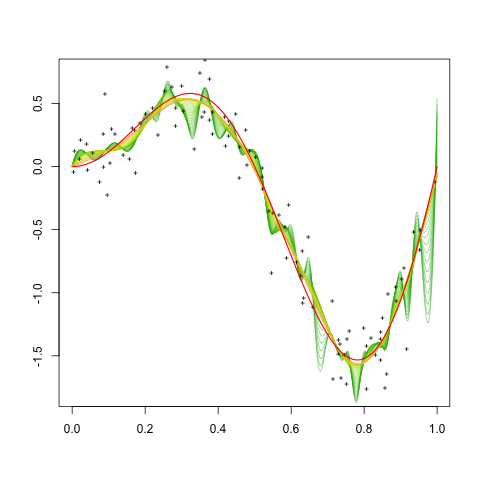
\includegraphics[scale=0.5]{PS_VCM_section_figure_3.png}
 \caption{$\hat{\mu}\left(t\right) = t \hat{\beta}\left(t\right)$}
\label{fig:PS_VCM_section_figure_2}
 \end{subfigure}
 \caption{\textit{Estimated coefficient function} $\hat{\beta}\left(t\right)$ \textit{and mean curve} $\hat{\mu}\left(t\right) = t \sin(2 \pi t)$ \textit{using a 80 B-splines basis functions of order 5 and a difference penalty of order} $k=3$.}
\end{figure}

The properties discussed in Section~\ref{BS_properties_continued} allude to how controlling the coefficients of a spline $f \in \mathscr{S}_{k,t}$ influences the shape of the overall function. Specifically, the form of the $j^{th}$ derivative provides an avenue of understanding how the differenced B-spline coefficient sequence is related to the volatility of the function on a given interval of its domain. The following figure visually explore the impact of the squared distance on adjacent basis coefficients on the function; a useful way of examining at P-splines is to consider the coefficients as the skeleton of the function, then draping the B-splines over them to put the flesh over the bones. A smoother sequence of coefficients leads to a smoother curve, which is clearly illustrated in Figure~\ref{fig:second_ord_PS_pen_SML_lambda}. As long as the coefficient sequence is smooth, the number of basis functions (and coefficients) is unimportant. The penalty ensures the smoothness of the skeleton.

\begin{figure}[H]
\begin{subfigure}{.5\textwidth}
  \centering
   \graphicspath{{img/}}
  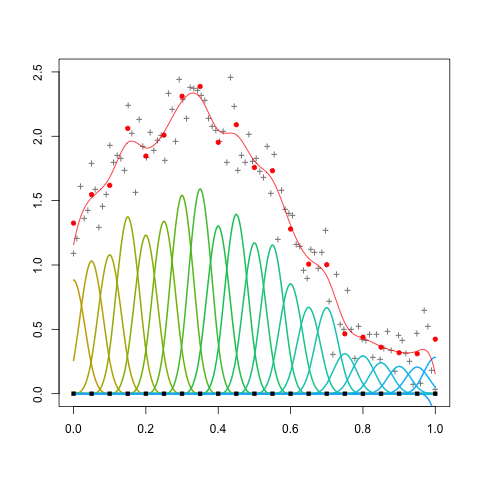
\includegraphics[scale=0.5]{pspline_pord2_xsmall_lambda.png}
  \label{fig:pspline_small_lambda}
\end{subfigure}
\begin{subfigure}{.5\textwidth}
  \centering
   \graphicspath{{img/}}
  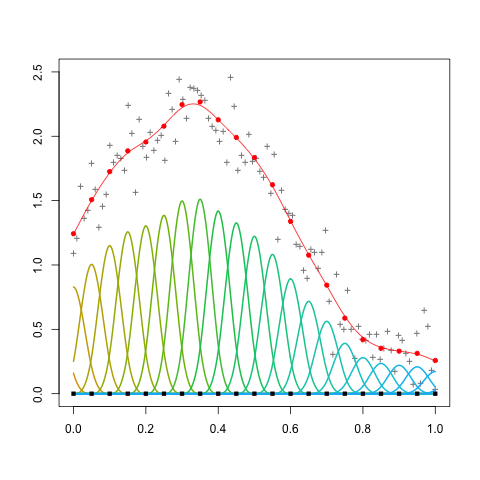
\includegraphics[scale=0.5]{pspline_pord2_small_lambda.png}
  \label{fig:pspline_small_lambda}
\end{subfigure}
\begin{subfigure}{.5\textwidth}
  \centering
   \graphicspath{{img/}}
  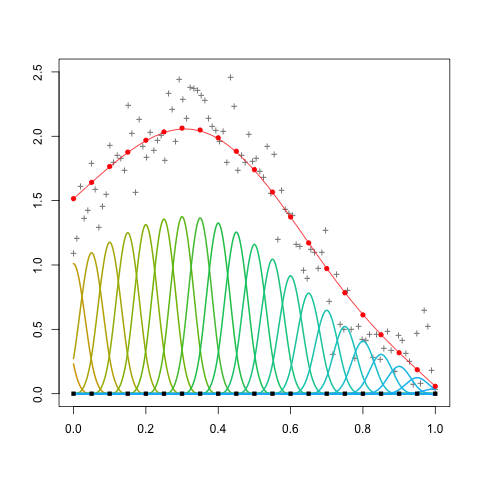
\includegraphics[scale=0.5]{pspline_pord2_medium_lambda.png}
  \label{fig:pspline_small_lambda}
\end{subfigure}
\begin{subfigure}{.5\textwidth}
  \centering
   \graphicspath{{img/}}
  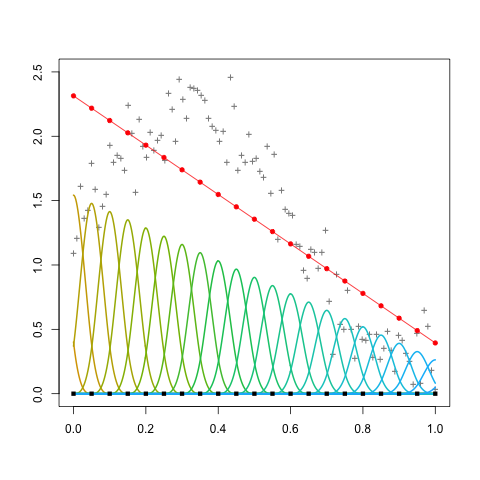
\includegraphics[scale=0.5]{pspline_pord2_large_lambda.png}
  \label{fig:pspline_small_lambda}
\end{subfigure}
\caption{\textit{Illustration of the impact of the second order difference penalty. The number of B-splines used is the same in each plot, with the value of the penalty parameter increasing from left to right and top to bottom across each plot. The fitted curve in the upper left plot is the most ``wiggly'' of any of the fits, as the penalty plays the weakest roll in the fitted coefficients there. The red circles are the values of each of the B-spline coefficients; as the penalty increases, they form as smoother sequence as we move across the four plots, which results in a smoother fitted function. As the penalty parameter approaches infinity, the fit approaches a linear function as shown in the bottom right plot.}}
\label{fig:second_ord_PS_pen_SML_lambda}
\end{figure}

The number of B-splines can be much larger than the number of observations because penalty ensures that the fitting procedure well-conditioned. One could literally use a thousand splines to fit ten observations without problems. Figure~\ref{fig:overcomplete_basis_pspline} illustrates this utility of the penalty for simulated data. There are $m=10$ observations and $40 + 3$ cubic B-splines. This property of P-splines cannot be overly appreciated, as it allows us to completely circumvent the nontrivial task of the optimal selection of knot placement. But one simply cannot have too many B-splines. Unless computational constraints are of concern, which is possible with large models, it is prudent to use even more. Figure~\ref{fig:PS_penalty_section_figure_3} shows how the fitted function changes as the tuning parameter $\lambda$ is varied in the presence of sparsely sampled data. 

\begin{figure}[H]   \label{fig:overcomplete_basis_pspline}
  \centering
   \graphicspath{{img/}}
  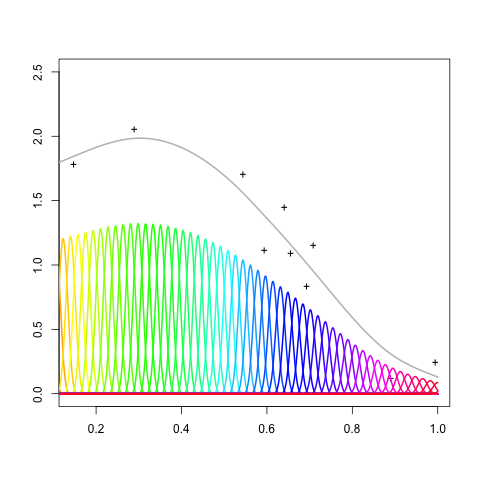
\includegraphics[scale=0.75]{pspline_10obs_60_basis_functions.png}
  \caption{P-spline smoothing of 10 observations using 60 B-spline basis functions.}
\end{figure}

\begin{figure}[H] \label{fig:PS_penalty_section_figure_3}
\centering
 \graphicspath{{img/}}
  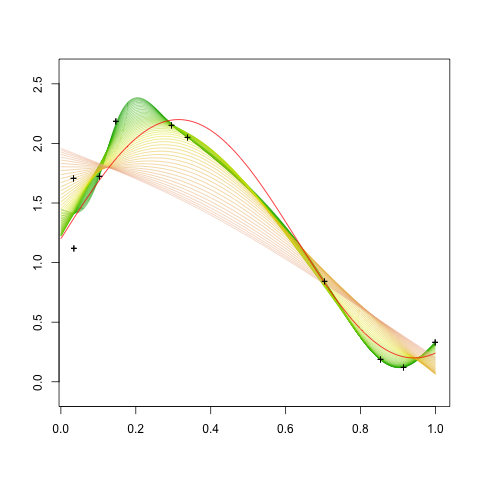
\includegraphics[width=4in, height=4in]{PS_penalty_section_figure_3.png}

  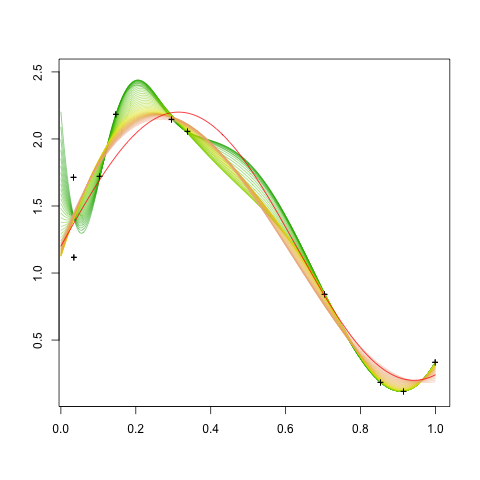
\includegraphics[width=4in, height=4in]{PS_penalty_section_figure_4.png}
 \caption{Fitted mean curves using a second (top) and third (bottom) order difference penalty for simulated data, sparsely sampled along the indexing variable: $y\left(t\right) = 1.2 + \sin\left(5t\right) + 0.2\epsilon_t$, where $\epsilon_t \stackrel{i.i.d.}{\sim}\textup{N}\left(0,1\right)$. A total of 10 data points were fit using a basis of 60 B-splines of degree $k=3$.}
\end{figure}